\section{Introdução aos Controladores Lógicos Programáveis (CLPs)}

\begin{frame}{Introdução}
	\begin{block}{}
		O CLP (Controlador Lógico Programável) é o \textbf{cérebro} de um processo industrial, sendo responsável por mantê-lo \textbf{funcionando de acordo com padrões pré-estabelecidos, informar falhas} e \textbf{cessar a operação da planta}, se necessário.
	\end{block}

	\centering
	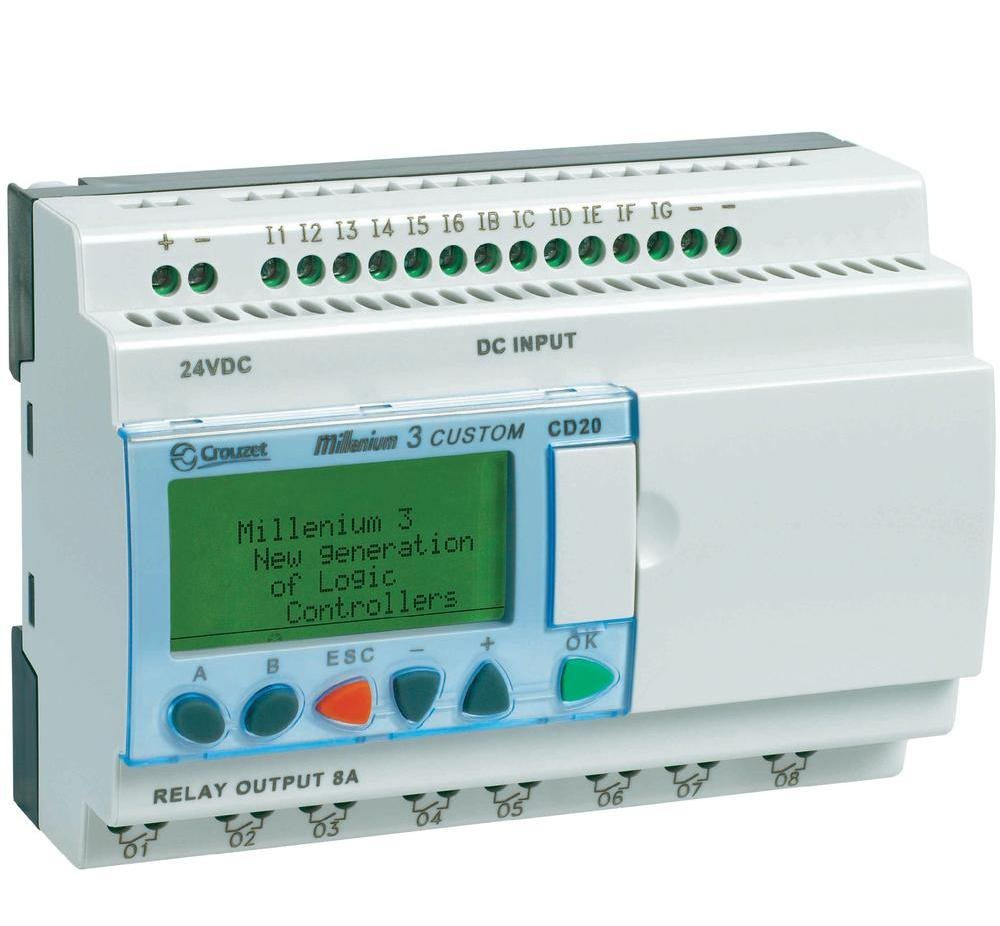
\includegraphics[width=0.5\linewidth]{Figuras/Ch08/fig1}

\end{frame}


\begin{frame}{Introdução}
	\begin{block}{Histórico}
		\begin{itemize}
			\item Antes do CLP eram necessários \textbf{vários técnicos} e \textbf{mão de obra especializada} para a montagem de \textbf{painéis elétricos} que realizassem as funções requeridas num \textbf{processo de montagem}.
			\item Havia um \textbf{grande descontentamento} no uso de \textbf{relés} em \textbf{todos} os ramos manufatureiros das indústrias, já que eram sistemas elétricos muito \textbf{custosos} e \textbf{ineficientes}.
		\end{itemize}
	\end{block}

	\centering
	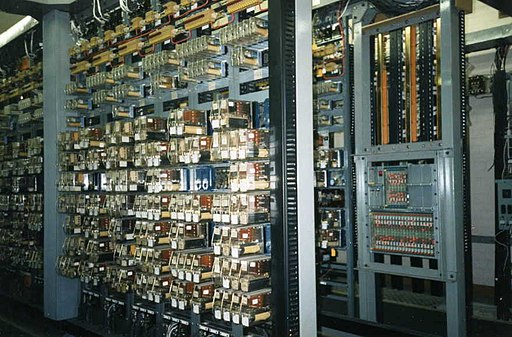
\includegraphics[width=0.55\linewidth]{Figuras/Ch08/fig3}
\end{frame}


\begin{frame}{Introdução}
	\begin{block}{Histórico}
		\begin{itemize}
			\item Os sistemas montados em painéis elétricos requeriam \textbf{manutenção frequente}, levando de \textbf{horas} até \textbf{dias} para trocar \textbf{uma bobina} curtada.
			\item Para \textbf{mudar a operação} de uma linha de montagem a fim de \textbf{alterar o produto final} era comum que uma fábrica \textbf{cessasse suas operações durante mais de um mês}, pois precisavam \textbf{refazer} todo o sistema elétrico.
		\end{itemize}
	\end{block}
	
	\centering
	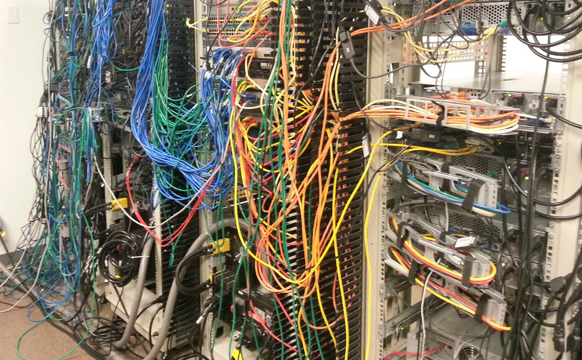
\includegraphics[width=0.5\linewidth]{Figuras/Ch08/fig4}
\end{frame}


\begin{frame}{Introdução}
	\begin{block}{Histórico}
		Numa nota oficial lançada no dia de ano novo de 1968 pela \textit{Hydra-Matic}, uma subdivisão da empresa General Motors, os engenheiros da companhia \textbf{detalharam o que seria necessário} em um ``controlador de máquinas padrão'':
		\begin{itemize}
			\item Um sistema de \textbf{estado sólido} (sem partes móveis) que fosse \textbf{flexível} como um computador, com \textbf{preço competitivo} e lógica de operação \textbf{similar a um sistema elétrico} de contatores.
			\item Fácil de ser \textbf{mantido} e \textbf{programado}.
			\item Capaz de trabalhar num \textbf{ambiente fabril}, com graxa, sujeira, umidade e eletromagnetismo.
			\item \textbf{Modular}, para facilitar a \textbf{manutenção} e \textbf{expansibilidade}.
		\end{itemize}
	\end{block}
\end{frame}


\begin{frame}{Introdução}
	\begin{block}{Histórico}
		Seguindo esses requisitos, várias empresas tentaram produzir o primeiro CLP.
	\end{block}

	\centering
	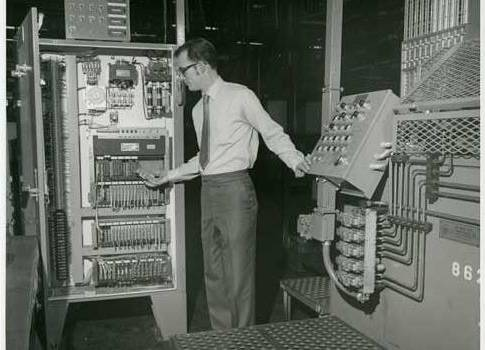
\includegraphics[width=0.7\linewidth]{Figuras/Ch08/fig2}

\end{frame}


\begin{frame}{Introdução}
	\begin{block}{Histórico}
		A empresa Modicon foi a primeira a fazer CLPs de qualidade que foram adotados pela indústria.
	\end{block}
	
	\begin{minipage}{0.48\linewidth}
		\centering
		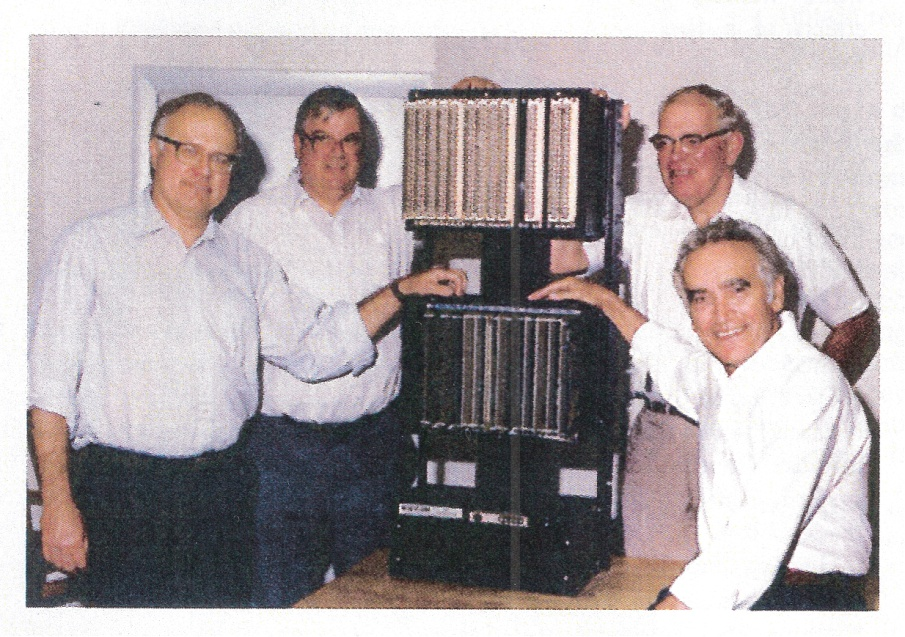
\includegraphics[width=1\linewidth]{Figuras/Ch08/fig5}
		
		\vspace{0.3cm}
		
		Modicon 084
	\end{minipage}
	\hfill
	\begin{minipage}{0.48\linewidth}
		\centering
		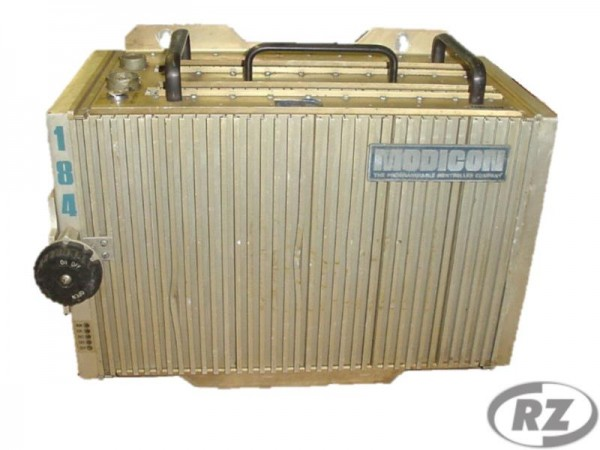
\includegraphics[width=1\linewidth]{Figuras/Ch08/fig6}
		
		Modicon 184
	\end{minipage}
\end{frame}


\begin{frame}{Construção}
	\begin{block}{Introdução}
		\begin{itemize}
			\item O CLP é muito similar a um computador, utilizando transistores e partes de estado sólido para realizar operações lógicas.
		\end{itemize}
	\end{block}

	\centering
	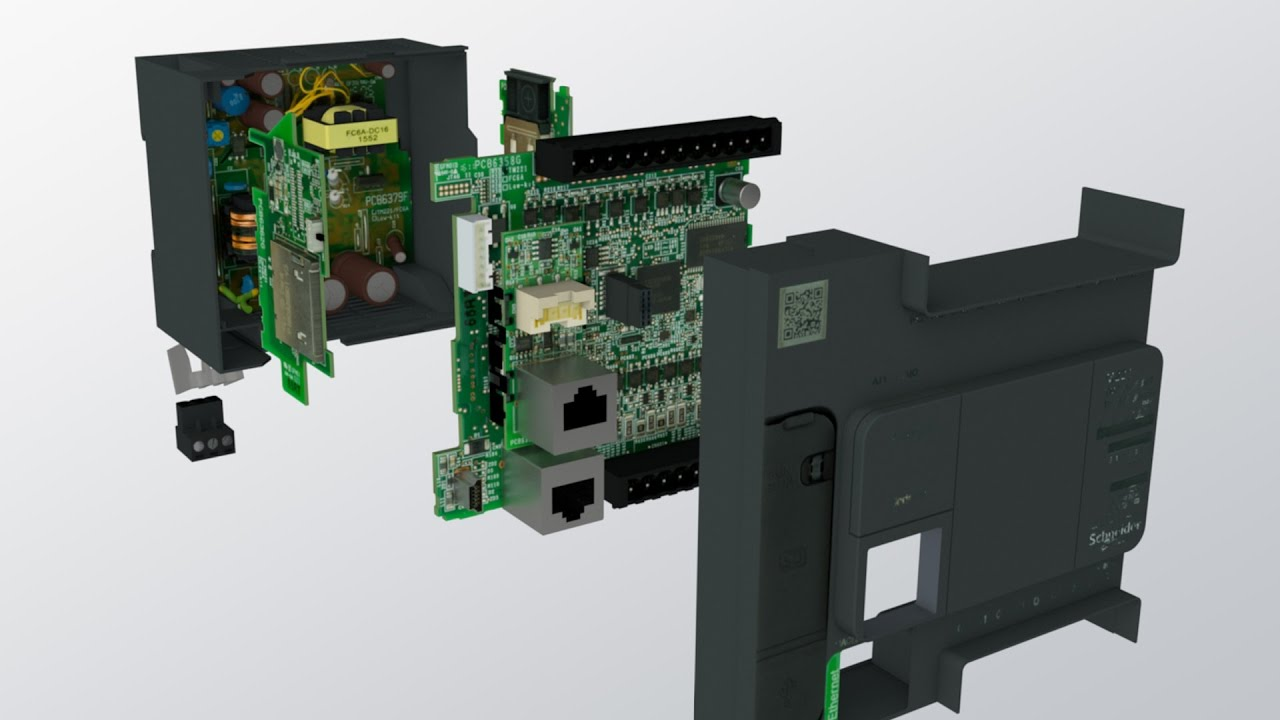
\includegraphics[width=0.8\linewidth]{Figuras/Ch08/fig7}
\end{frame}


\begin{frame}{Construção}
	
	\centering
	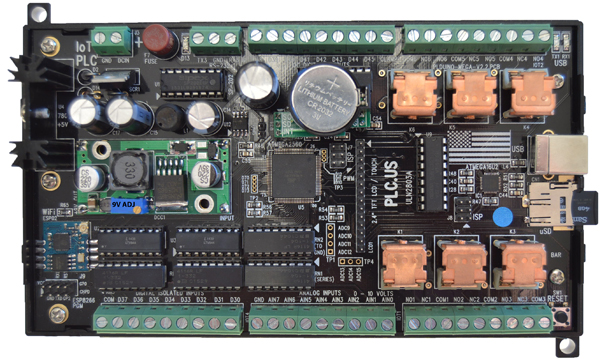
\includegraphics[width=0.8\linewidth]{Figuras/Ch08/fig8}
	
	Circuito de um CLP real
\end{frame}


\begin{frame}{Construção}
	\begin{block}{Arquitetura}
		\begin{itemize}
			\item O CLP possui uma arquitetura de acordo com o diagrama de blocos abaixo.
		\end{itemize}
	\end{block}
	
	\centering
	
	\begin{tikzpicture}[scale=0.5]
			\draw (-4,-3) rectangle (4,3); %CLP
		\draw (-4,0) -- (-2.5,0); %Div in out
		\draw (-2.5,-3) -- (-2.5,3); %Div cartoes
		\draw (-1.5,-2.5) rectangle (0,2.5); %Mem dados
		\draw (0.5,-2.5) rectangle (3.5,-1); %Mem prog
		\draw (1,0) rectangle (3,2); %CPU
		\draw (-4,-5) rectangle (4,-3); %Alimentacao
		\draw (-2.5,4) rectangle (4,6); %Term de prog
		
		\draw (1,2.6) node {CLP};
		
		\draw (-3.25,1.5) node[text width=1.5cm,align=center,rotate=90] {\small Cartões de input};
		
		\draw (-3.25,-1.5) node[text width=1.5cm,align=center,rotate=90] {\small Cartões de output};
		
		\node at (2,1) {\small CPU};
		
		\node[rotate=90,text width=1.5cm,align=center] at (-0.75,0) {\small Memória de dados};
		
		\node[text width=2cm,align=center] at (2,-1.75) {\footnotesize Memória de programa};
		
		\node at (-6,0) {Campo};
		
		\node at (0,-4) {Alimentação};
		
		\node[text width=3cm,align=center] at (0.75,5) {Terminal de programação};
		
		\draw[-Latex] (-8,1.5) -- node[above] {Entradas} +(4,0);
		\draw[Latex-] (-8,-1.5) -- node[below] {Saídas} +(4,0);
		\draw[-Latex] (-2.5,1.5) -- +(1,0);
		\draw[Latex-] (-2.5,-1.5) -- +(1,0);
		\draw[-Latex] (0,1.5) -- +(1,0);
		\draw[Latex-] (0,0.5) -- +(1,0);
		\draw[Latex-] (2,0) -- +(0,-1);
		
		\draw[-Latex] (-1.5,4) -- +(0,-1);
		\draw[Latex-] (3,4) -- +(0,-1);
	\end{tikzpicture}
\end{frame}


\begin{frame}{Construção}
	\begin{block}{Arquitetura}
		\begin{itemize}
			\item O \textit{Terminal de programação} é o meio de \textbf{acessar o CLP}, tanto para \textbf{operação corriqueira} quanto para \textbf{programação}.
		\end{itemize}
	\end{block}
	
	\vspace{0.2cm}
	
	\centering
	
	\begin{tikzpicture}[scale=0.5]
	\draw (-2.5,4) rectangle (4,6); %Term de prog
	
	\node[text width=3cm,align=center] at (0.75,5) {Terminal de programação};
	
	\draw[-Latex] (-1.5,4) -- +(0,-1);
	\draw[Latex-] (3,4) -- +(0,-1);
	
	\draw (-2.5,2) -- ++(0,1) -- node[midway,below] {\small CLP} ++(6.5,0) -- +(0,-1);
	\end{tikzpicture}
\end{frame}


\begin{frame}{Construção}
	\begin{block}{Arquitetura}
		\begin{itemize}
			\item A \textit{Alimentação} do CLP e dos cartões é sua fonte de energia, que deve ser \textbf{estável} e \textbf{continua}.
			\item Normalmente, o CLP possui uma \textbf{bateria interna}, que deve \textbf{salvar} o \textbf{programa carregado} e seu \textbf{estado}.
			\item Essa bateria interna, com frequência, é um \textbf{``super-capacitor''}.
		\end{itemize}
	\end{block}
	
	\vspace{0.2cm}
	
	\centering
	
	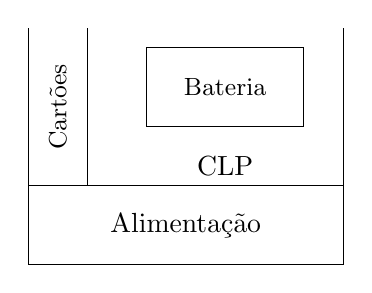
\begin{tikzpicture}[scale=0.5]
	\draw (-4,1) -- (-4,-3) -- (4,-3) -- (4,1); %CLP
	\draw (-2.5,-3) -- (-2.5,1); %Div cartoes
	\draw (-4,-5) rectangle (4,-3); %Alimentacao
	
	\draw (1,-3) node[above] {CLP};
	
	\draw (-3.25,-1) node[rotate=90] {\small Cartões};
	
	\draw (-1,-1.5) rectangle (3,0.5);
	
	\node at (0,-4) {Alimentação};
	\draw (1,-0.5) node {\small Bateria};
	\end{tikzpicture}
\end{frame}


\begin{frame}{Construção}
	\begin{block}{Arquitetura}
		\begin{itemize}
			\item O \textit{Campo} é o \textbf{chão de fábrica}, onde ocorre o processo.
			\item A função do CLP é supervisionar e controlar o que ocorre no campo.
			\item Os sinais do campo, geralmente enviados em forma de corrente de $ 4 $ a \SI{20}{\milli\ampere}, precisam ser \textbf{convertidos} para binário, que é a linguagem do CLP, e depois de volta para sinais elétricos.
			\item Os \textbf{cartões} de entrada e saída realizam essa função.
		\end{itemize}
	\end{block}
	
	\vspace{0.2cm}
	
	\centering
	
	\begin{tikzpicture}[scale=0.5]
	\draw (-1.5,-3) -- (-4,-3) -- (-4,3) -- (-1.5,3); %CLP
	\draw (-4,0) -- (-2.5,0); %Div in out
	\draw (-2.5,-3) -- (-2.5,3); %Div cartoes
	
	\draw (-2.5,0) node[right] {CLP};
	
	\draw (-3.25,1.5) node[text width=1.5cm,align=center,rotate=90] {\small Cartões de input};
	
	\draw (-3.25,-1.5) node[text width=1.5cm,align=center,rotate=90] {\small Cartões de output};
	
	\node at (-6,0) {Campo};
	
	\draw[-Latex] (-8,1.5) -- node[above] {Entradas} +(4,0);
	\draw[Latex-] (-8,-1.5) -- node[below] {Saídas} +(4,0);

	\end{tikzpicture}
\end{frame}


\begin{frame}{Construção}
	\begin{block}{Arquitetura}
		\begin{itemize}
			\item O CLP possui \textbf{diversos} internos que serão abordados mais a frente, e que trabalham em conjunto para seu funcionamento devido.
		\end{itemize}
	\end{block}
	
	\vspace{0.2cm}
	
	\centering
	
	\begin{tikzpicture}[scale=0.5]
	\draw (-4,-3) rectangle (4,3); %CLP
	\draw (-4,0) -- (-2.5,0); %Div in out
	\draw (-2.5,-3) -- (-2.5,3); %Div cartoes
	\draw (-1.5,-2.5) rectangle (0,2.5); %Mem dados
	\draw (0.5,-2.5) rectangle (3.5,-1); %Mem prog
	\draw (1,0) rectangle (3,2); %CPU
	
	\draw (1,2.6) node {CLP};
	
	\draw (-3.25,1.5) node[text width=1.5cm,align=center,rotate=90] {\small Cartões de input};
	
	\draw (-3.25,-1.5) node[text width=1.5cm,align=center,rotate=90] {\small Cartões de output};
	
	\node at (2,1) {\small CPU};
	
	\node[rotate=90,text width=1.5cm,align=center] at (-0.75,0) {\small Memória de dados};
	
	\node[text width=2cm,align=center] at (2,-1.75) {\footnotesize Memória de programa};
	
	\node at (-6,0) {Campo};
	
	\draw[-Latex] (-8,1.5) -- node[above] {Entradas} +(4,0);
	\draw[Latex-] (-8,-1.5) -- node[below] {Saídas} +(4,0);
	\draw[-Latex] (-2.5,1.5) -- +(1,0);
	\draw[Latex-] (-2.5,-1.5) -- +(1,0);
	\draw[-Latex] (0,1.5) -- +(1,0);
	\draw[Latex-] (0,0.5) -- +(1,0);
	\draw[Latex-] (2,0) -- +(0,-1);
	\end{tikzpicture}
\end{frame}


\begin{frame}{Memória}
	\begin{block}{Introdução}
		\begin{itemize}
			\item As memórias são uma das \textbf{principais partes} do CLP, e devem guardar dados \textbf{provisória} ou \textbf{permanentemente}.
			\item Chamamos as memórias ``provisórias'' de \textbf{voláteis} ou \textbf{não-retentivas}, pois dependem de uma \textbf{fonte constante} para guardar seu estado.
			\item As memórias ``permanentes'' são chamadas \textbf{não voláteis} ou \textbf{retentivas}.
			\item As memórias guardam dados em forma de \textbf{estados lógicos} (V ou F, 0 ou 1) ou \textbf{conjuntos de estados}. 
			\item Cada tipo de dado recebe um nome de acordo com seu \textbf{tamanho}.
		\end{itemize}
	\end{block}
	
	\centering
	
	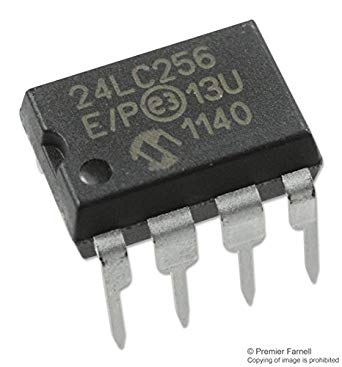
\includegraphics[height=0.3\textheight]{Figuras/Ch08/fig10}
	
\end{frame}


\begin{frame}{Memória}
	\begin{block}{Tipos de dados}
		\begin{itemize}
			\item O menor tipo de dado dado possível é um \textbf{bit}, que se trata de um único estado lógico.
			\item Depois temos os quartetos, chamados de \textbf{nibbles}.
			\item Os octetos, que são o formato padrão de dados, chamado \textbf{byte}.
			\item As \textbf{words}, que possuem 16 bits em sequência.
		\end{itemize}
	\end{block}
	
	\centering
	
	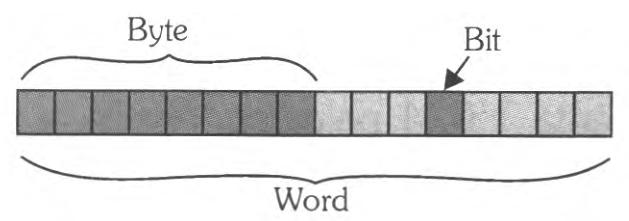
\includegraphics[width=0.7\linewidth]{Figuras/Ch08/fig9}
	
\end{frame}


\begin{frame}{Memória}
	\begin{block}{Tipos de memórias}
		\begin{itemize}
			\item Além dessas temos \textbf{double words} e outros tipos de dados que são baseados em potências de 2.
			\item Vale notar que nos computadores, geralmente, temos \textbf{outros nomes} para a \textbf{mesma quantidade de bits}, mas que servem para distinguirmos o \textbf{tipo de dado guardado} (número inteiro, letra, número real).
		\end{itemize}
	\end{block}
	
	
	
\end{frame}


\begin{frame}{Memória - Tipos de dados I}
	\renewcommand{\arraystretch}{1.2}
	\resizebox{\textwidth}{!}{%
	\begin{tabular}{cccc}
		\toprule
		\thead{\normalsize Tipo de \\ 
			\normalsize dado} & Descrição 			& \thead{\normalsize Tamanho \\ 
										\normalsize (em bits)} 	& Range\\ \midrule
		BOOL 	& \makecell{
				\textit{Boolean}\\
				Falso ou Verdadeiro} 	& 1 		& \multirow{5}{*}{$ \begin{aligned}
													0 \text{ }&\text{ou }1\\[0.85em]
													-(2^{7})&\sim(2^{7}-1)=\\
													\num{-128}&\sim127\\[-0.1em]
													-(2^{15})&\sim(2^{15}-1)=\\
													\num{-32768}&\sim\num{32767}\\[0.2em]
													-(2^{31})&\sim(2^{31}-1)= \\
													\num{-2147438648}&\sim\num{2147438647}\\[1em]
													0&\sim(2^{8}-1)= \\
													0&\sim255
													\end{aligned} $} \\ \midrule
		SINT 	& \makecell{
				\textit{Short Integer}\\ 
				Número inteiro curto} 	& 8 		& \\ \midrule
		INT 	& \makecell{
				\textit{Integer}\\ 
				Número inteiro} 		& 16 		& \\ \midrule
		DINT 	& \makecell{
				\textit{Double Integer}\\ 
				Número inteiro de\\
				dupla precisão} 		& 32 		& \\ \midrule
	\makecell{
		USINT \\
		BYTE} & \makecell{
				\textit{Unsigned Short Integer}\\ 
				Número inteiro curto \\
				sem sinal} 				& 8 		& \\ \bottomrule
	\end{tabular}}
\end{frame}


\begin{frame}{Memória - Tipos de dados II}
	\renewcommand{\arraystretch}{1.2}
	\resizebox{\textwidth}{!}{%
	\begin{tabular}{cccc}
		\toprule
		\thead{\normalsize Tipo de \\ 
			\normalsize dado} & Descrição 			& \thead{\normalsize Tamanho \\ 
			\normalsize (em bits)} 	& Range\\ \midrule
	\makecell{
		UINT \\ 
		WORD} & \makecell{
		\textit{Unsigned Integer}\\ 
		Número inteiro \\
			sem sinal} 				& 16 		& \multirow{5}{*}{\smash{\raisebox{-5.2em}{$ 
													\begin{aligned}
													0&\sim(2^{16}-1)= \\
													0&\sim\num{65535} \\[1.7em]
													0&\sim(2^{32}-1)= \\
													0&\sim\num{4294967295}\\[1.8em]
													\text{Ver }&\text{Norma IEEE-754}\\[2em]
													\text{Ver }&\text{Norma IEEE-754}\\[1.3em]
													0&\sim(2^{32}-1)\,\si{\milli\second}= \\
													0&\sim\SI{4294967295}{\milli\second}
													\end{aligned} $}}} \\ \midrule
	\makecell{
		UDINT \\ 
		DWORD} & \makecell{
		\textit{Unsigned Double Integer}\\
		Número inteiro de\\
		dupla precisão \\
		sem sinal} 				& 32 		& \\ \midrule
	\makecell{
		REAL \\ 
		FLOAT} & \makecell{
		\textit{Floating Point Number}\\
		Números reais} 			& 32 		& \\ \midrule
	\makecell{
		LREAL \\ 
		LFLOAT} & \makecell{\textit{Long Real/Double Float}\\
		Números reais de\\
		dupla precisão} 		& 64 		& \\ \midrule
	TIME 	& \makecell{
		\textit{Time}\\
		Período (em \si{\milli\second})} & 32 & \\ \bottomrule
	\end{tabular}}
\end{frame}


\begin{frame}{Memória}
	\begin{block}{Prefixos}
		\begin{itemize}
			\item Até agora vimos dados em unidade, isto é, \textbf{um} byte ou \textbf{uma} word.
			\item No mundo real esses dados \textbf{raramente} estão soltos em unidades e, frequentemente, encontramos grupos \textbf{muito grandes} deles.
			\item Assim como quando medimos mil metros e colocamos o prefixo \textit{quilo} para indicar isso, podemos dizer que, quando medimos 1024 ($ 2^{10} $) de um tipo de dados isso equivale a \textbf{um quilo} do tipo de dado.
			\item Por exemplo, 1024 bytes equivale a \textbf{um \textit{quilo}byte}.
			\item Assim como no exemplo de metros, podemos abreviar \textit{quilobyte} por \si{\kilo\byte}.
		\end{itemize}
	\end{block}
\end{frame}


\begin{frame}{Memória}
	\begin{block}{Prefixos}
		Alguns prefixos comuns são:
		\begin{itemize}
			\item \textit{Mega} (M) para \SI{1024}{\kilo\byte}.
			\item \textit{Giga} (G) para \SI{1024}{\mega\byte}.
			\item \textit{Tera} (T) para \SI{1024}{\giga\byte}.
			\item \textit{Peta} (P) para \SI{1024}{\tera\byte}.
		\end{itemize}
	\end{block}
\end{frame}


\frame{
	\frametitle{Exercícios}
	\begin{block}{}
		01. Você consegue imaginar como o CLP entende a entrada de um pressostato (chave de pressão)? Explique.
		
		\vspace{0.5cm}
		
		02. Cite exemplos de aplicações do CLP em coisas do seu dia a dia. Você gostaria de automatizar algum processo na sua rotina com o CLP?
		
		\vspace{0.5cm}
		
		03. Numa indústria, um CLP possui \SI{256}{\mega\byte} de memória. Isso vale quantos \textbf{bits} de memória?
	\end{block}
}

\section*{Referências}
\frame{
	\frametitle{Referências e Exercícios Complementares}
	\begin{itemize}
		\item FRANCHI, Claiton Moro; CAMARGO, Valter Luis Arlindo de. Controladores Lógicos Programáveis - Sistemas Discretos, 1 ed. Érica, 2008.
		\item TAVARES, Leonardo; MONTEIRO, Natália Nogueira. Controladores Lógicos Programáveis, 1 ed. [s.n.], 2017.
	\end{itemize}
	%\centering{\alert{Página 546 - \textbf{Capítulo 6}}} \\
	%\centering{\alert{Lista de exercícios 01}}
}